%%%From presentation Aarhus, 11 October 2017


\documentclass[12pt, notes=show]{beamer}

\usetheme[width=0cm]{Goettingen}
\usecolortheme{rose}
\useoutertheme{default}
\setbeamerfont{caption}{size=\scriptsize}
\setbeamertemplate{navigation symbols}{}

%%change default colors
\definecolor{UPF}{RGB}{200,16,46}
\setbeamercolor{title}{fg=UPF}
\setbeamercolor{frametitle}{fg=UPF}
\setbeamercolor{structure}{fg=UPF}

%%To remove upper and lower beamer pane and add number of page
\addtobeamertemplate{navigation symbols}{}{%
	\usebeamerfont{footline}%
	\usebeamercolor[fg]{footline}%
	\hspace{1em}%
	$\dfrac{\insertframenumber}{\inserttotalframenumber}$
}

\usepackage{hyperref}
\usepackage{fontspec} 
\setsansfont{Futura LT}

\usepackage{array}

\usepackage{arydshln}
\usepackage{amsmath}

\usepackage{mathptmx}
\usepackage{latexsym}
\usepackage{mathtools}
\usepackage{multirow}
\usepackage{caption}
\usepackage{listings}
\usepackage{algorithm,algorithmicx,algpseudocode}

\algnewcommand\And{\textbf{and}}

\DeclarePairedDelimiter\abs{\lvert}{\rvert}%
\DeclarePairedDelimiter\norm{\lVert}{\rVert}%

\newcommand{\specialcell}[2][c]{%
  \begin{tabular}[#1]{@{}c@{}}#2\end{tabular}}


\makeatletter
\let\oldabs\abs
\def\abs{\@ifstar{\oldabs}{\oldabs*}}
\let\oldnorm\norm
\def\norm{\@ifstar{\oldnorm}{\oldnorm*}}
\makeatother
\usepackage[beamer,customcolors]{hf-tikz}
\usepackage{tabularx}
\usepackage{colortbl}

%%Tikz command used to annotate table
%
\newcounter{nodecount}

\newcolumntype{g}{>{\columncolor{red}}c}

\newcommand\tabnode[1]{%
    \addtocounter{nodecount}{1}%
    \tikz[remember picture,overlay]\node[inner sep=0pt] (\thenodecount) {#1};}
%
%%%%%%%%%%



\title{
	An agent-based model of trade in the Roman East (25BC-150AD) \\
	{\small Impact of social interactions on economic trends}
}

\institute{UrbNet seminar series\\ Aarhus, Octobre 2017}

\author{Simon Carrignon, Tom Brughmans \& Iza Romanowska}

\date{
	\scriptsize
	\begin{columns}
		\begin{column}{.3\textwidth}
			\begin{center}
				
\includegraphics[height=1cm]{../../logos/bscLogo.jpg} \hspace{2cm}
			\end{center}
		\end{column}
		\begin{column}{.3\textwidth}
			\begin{center}
				
\includegraphics[height=1cm]{../../logos/upf_word_imp.jpg} %declare logo image with an alias here 
			\end{center}
		\end{column}
	\end{columns}

}
\begin{document}



\begin{frame}
    \begin{algorithm}[H]
	\caption{Model}
	\label{algo:complete}
	\begin{algorithmic}[1]
	    \tiny
	    \State INITIALIZATION: 
	    \For{$i \in \#Pop$} \Comment{Initialize the agent with no goods and a random value vector}
	    \State $Q^i = (0, \cdots, 0)$
	    \State $V^i = (v^i_0, \cdots, v^i_n)$ \Comment{The values of $v^i_j$ are selected randomly}
	    \EndFor

	    \State SIMULATION:
	    \Loop{$~step \in TimeSteps$}
	    \For{$i \in Pop$}
	    \State $Production(Q^i)$
	    \EndFor
	    \For{$i \in Pop$}
	    \For{$j \in Pop$}
	    \State $TradeProcess(V^i,Q^i,V^j,Q^j)$
	    \EndFor		
	    \EndFor
	    \For{$i \in Pop$}
	    \State $ConsumeGoods(Q^i)$ \Comment{All goods are consumed}
	    \If{$ (step \mod CulturalStep) = 0$}	
	    \State $CulturalTransmission(V)$
	    \State $Innovation(V^i)$
	    \EndIf
	    \EndFor
	    \EndLoop
	\end{algorithmic}
    \end{algorithm}


\end{frame}
\begin{frame}{Consumption}
    
    Before : 
\begin{equation}
s^i_j = \begin{cases}
 s_{max}=1 & \text{if $q^i_j = n_j$}\\
1 -\dfrac{\abs{q^i_j - n_j}}{ \sqrt{\abs{(q^i_j)^2-(n_j)^2}}} & \text{if $q^i_j \neq n_j$}
\end{cases}
\end{equation}

\uncover<2->{ 
    
    Now
\begin{equation}
s^i_j = q^i_j 
\end{equation}
}

\end{frame}

\begin{frame}{Trade}
    
    %\begin{algorithm}
    %\caption{Trading Process for agent $o$}
    	\begin{algorithmic}[1]
    	\scriptsize
    		\For{$j \in Goods \And j \neq produced^o $}
    			\State $tradeAttempt = 0$
    			\For{$r \in Pop \And produced^r = j \And tradeAttempt < TradeThreshold $}
				\State $W_r = estimateNeeds() $
    				\If{$acceptableTrade(W_o,W_r)$}
    					\State $trade(W_o,W_r)$
    				\Else
    					\State $tradeAttempt = tradeAttempt+1$					
    				\EndIf
    			\EndFor
    		\EndFor
    \end{algorithmic}
    %\end{algorithm}

\end{frame}

\begin{frame}
    \center
    \includegraphics[height=6cm]{test.png} %declare logo image with an alias here 
\end{frame}

\begin{frame}{Experimental framework}

\textcolor{UPF}{\textbf{2.}\Huge}
\uncover<+->{Experimental setup, test the importance of those factors:}
    \begin{itemize}
	\item<+-> 	    \textbf{Individual learning}/creativity: ``a settlement decides to change the value of a ware''\\
	    \uncover<+->{$\mu \rightarrow$ increase the probability of creating a new solution\\}

	    \uncover<+->{\hspace{.2cm} $\mu \in \{0.001,0.01,0.1,1\}$}
	\item<+-> 	    \textbf{Social learning}/openness:``a market decide to copy another, more successful market''\\
	    \uncover<+->{$\lambda\rightarrow$ increase the probability to copy a more successful settlement\\}

	    \uncover<+->{\hspace{.2cm} $\lambda \in \{0.0001,0.001,0.01,0.1,1,10\}$}
	\item<+->  $ 6 \times 4 = 24$ setup, 50s simulation each
    \end{itemize}
\end{frame}


\begin{frame}{Result}
    1200 Simulations for different pairs of parameters.
    \begin{table}
	\centering

	\begin{tabular}{rr|cccc}
	    & &\multicolumn{4}{c}{ $\mu$ } \\
	    & & $0.001$ & $0.01$ & $0.1$ & $1$ \\ \hline
	    \multirow{6}{*}{$\lambda$} 
	    & 0.0001	& $\times50$ & $\times50$ & $\times50$ & $\times50$ \\
	    & 0.001	& $\times50$ & $\times50$ & $\times50$ & $\times50$ \\
	    & 0.01	& $\times50$ & $\times50$ & $\times50$ & $\times50$ \\
	    & 0.1	& $\times50$ & $\times50$ & $\times50$ & $\times50$ \\
	    & 1		& $\times50$ & $\times50$ & $\times50$ & $\times50$ \\
	    & 10	& $\times50$ & $\times50$ & $\times50$ & $\times50$ 
	\end{tabular}
    \end{table}

\end{frame}

\begin{frame}{Result}

    \tikzset{
	every picture/.style={remember picture,baseline},
	every node/.style={
	    inner sep=0pt,
	    anchor=base,
	    minimum width=1.8cm,
	    align=center,
	    text depth=.25ex,
	outer sep=1.5pt},
	every path/.style={
	    thick, 
	    rounded corners
	}
    }  
    1200 Simulations for different pairs of parameters.

    \begin{table}
	\center
	\begin{tabular}{rrcccc}
	    & &\multicolumn{4}{c}{ creativity } \\
	    & &\multicolumn{1}{|c}{\tiny $--$ } & \multicolumn{2}{c}{ \tiny \dots }& \tiny $++$ \\\cline{2-6}
	    \multirow{6}{*}{\rotatebox[origin=c]{90}{openness}} 
	    & \multirow{2}{*}{\tiny $--$}
	    		& \multicolumn{1}{|c}{$\times50$ } & $\times50$ & $\times50$ & $\times50$ \\
			& 		& \multicolumn{1}{|c}{$\times50$ } & $\times50$ & $\times50$ & \tabnode{$\times50$} \\
	    & \multirow{2}{*}{\tiny \dots}
	    		& \multicolumn{1}{|c}{$\times50$ } & $\times50$ & $\times50$ & $\times50$ \\
	    & 		& \multicolumn{1}{|c}{$\times50$ } & $\times50$ & $\times50$ & $\times50$ \\
	    & \multirow{2}{*}{\tiny $++$}
	    		& \multicolumn{1}{|c}{$\times50$ } & $\times50$ & $\times50$ & $\times50$ \\
			& 	& \multicolumn{1}{|c}{ \tabnode{$\times50$} } & $\times50$ & $\times50$ & $\times50$ 
	\end{tabular}
    \end{table}
\end{frame}

\begin{frame}{Exemple}
    \small
    \centering
    \begin{table}
	\begin{tabular}{ccc}
	    Data 	&  ExpG {\tiny ($\lambda=0.001,\mu=1$)} &  ExpB {\tiny ($\lambda=10,\mu=0.001$)}   \\
	    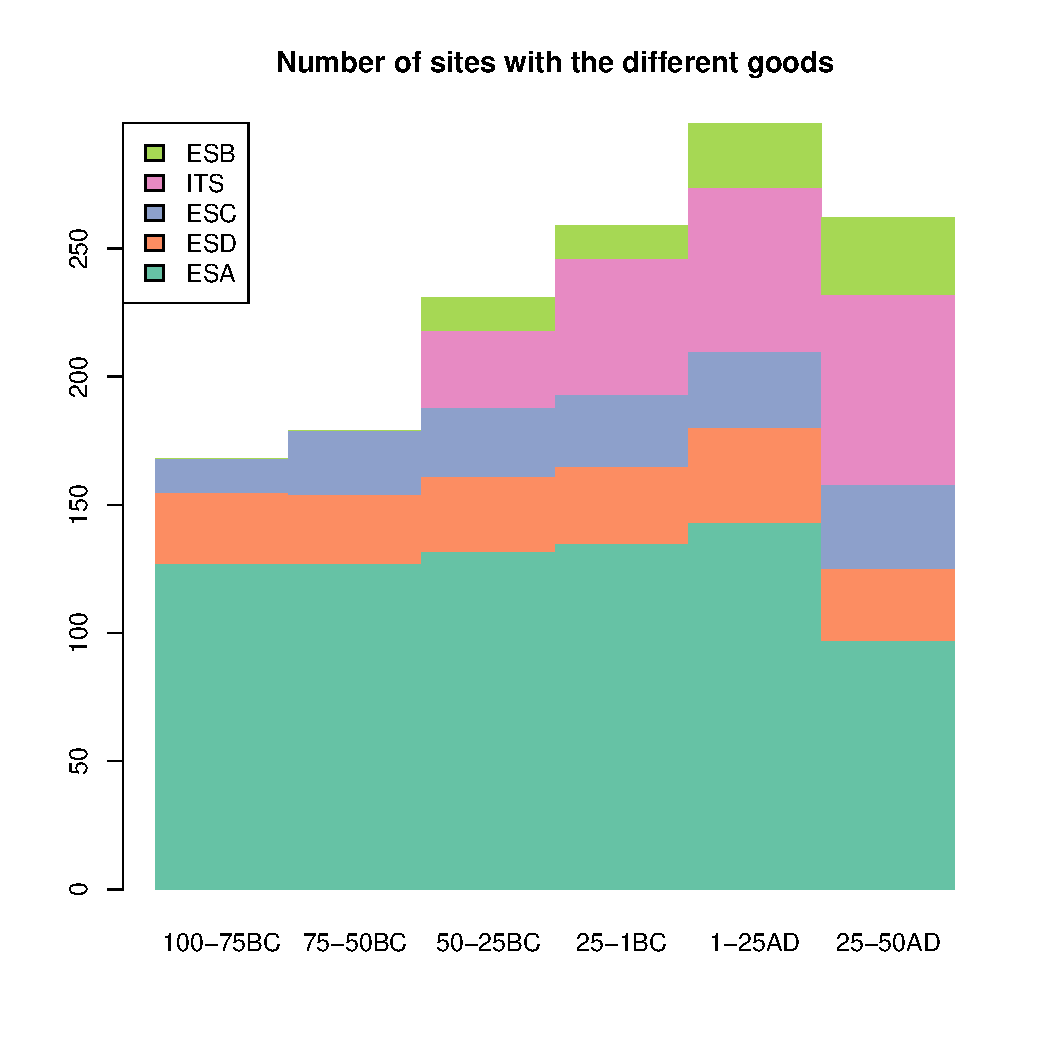
\includegraphics[width=.3\textwidth]{images/hmData.pdf}	&
	    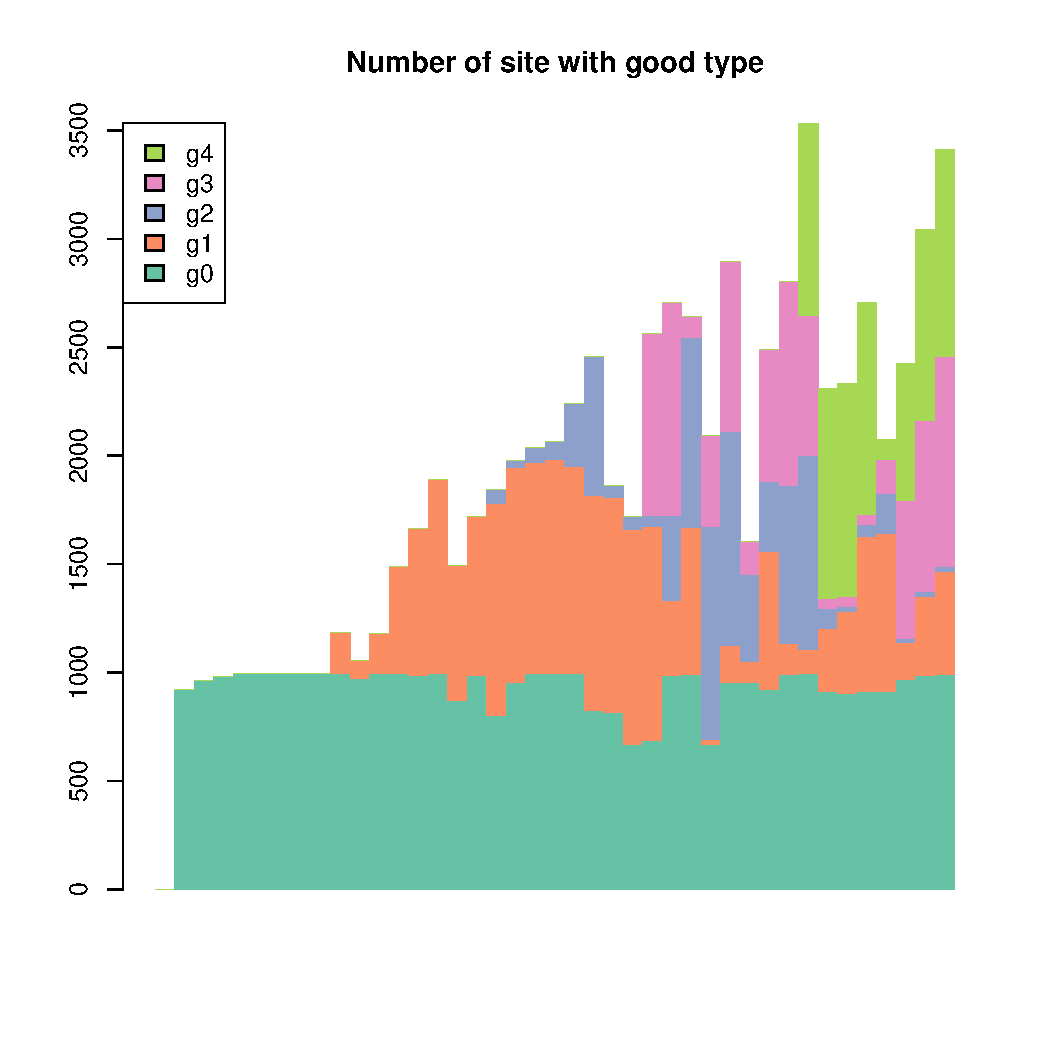
\includegraphics[width=.3\textwidth]{images/hmGoodSimu.pdf}	&
	    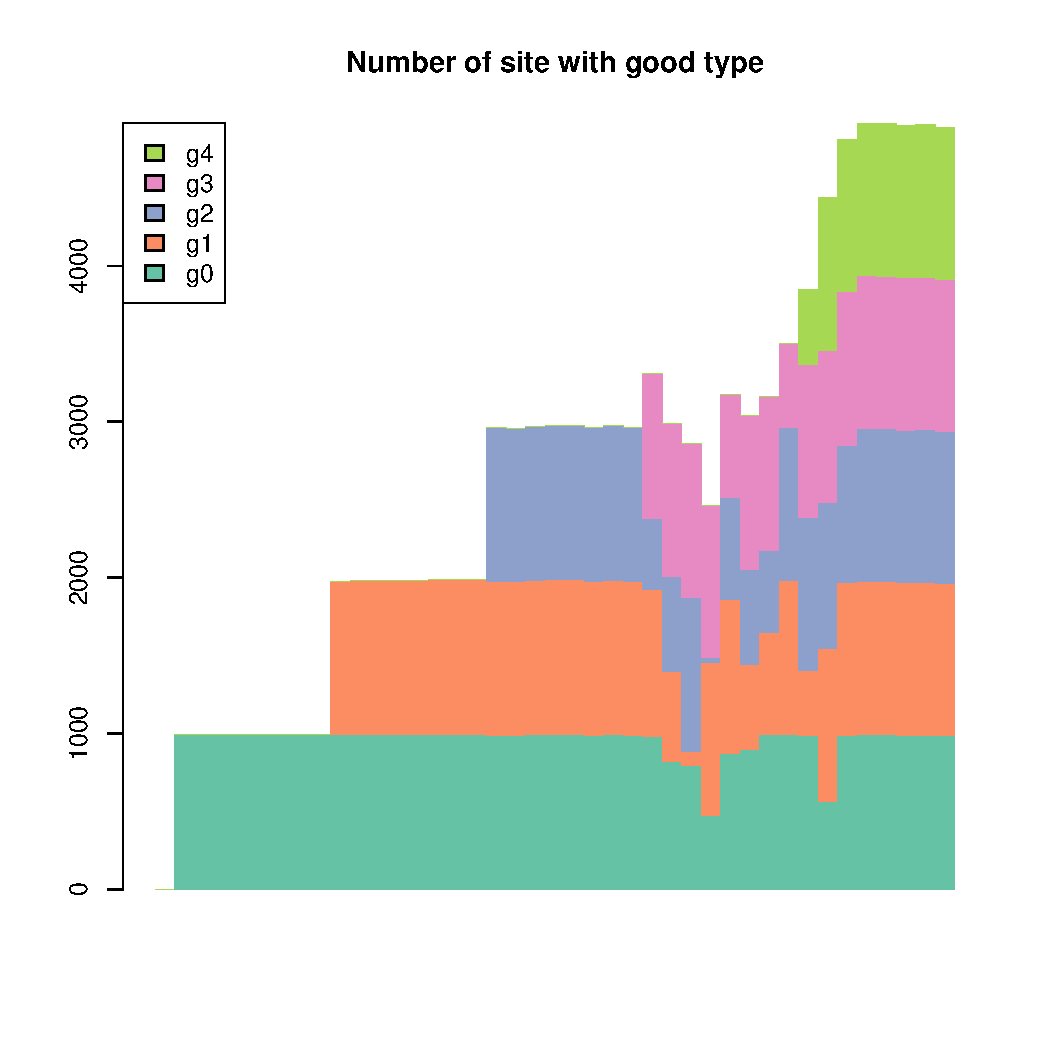
\includegraphics[width=.3\textwidth]{images/hmBadSimu.pdf}	\\
	    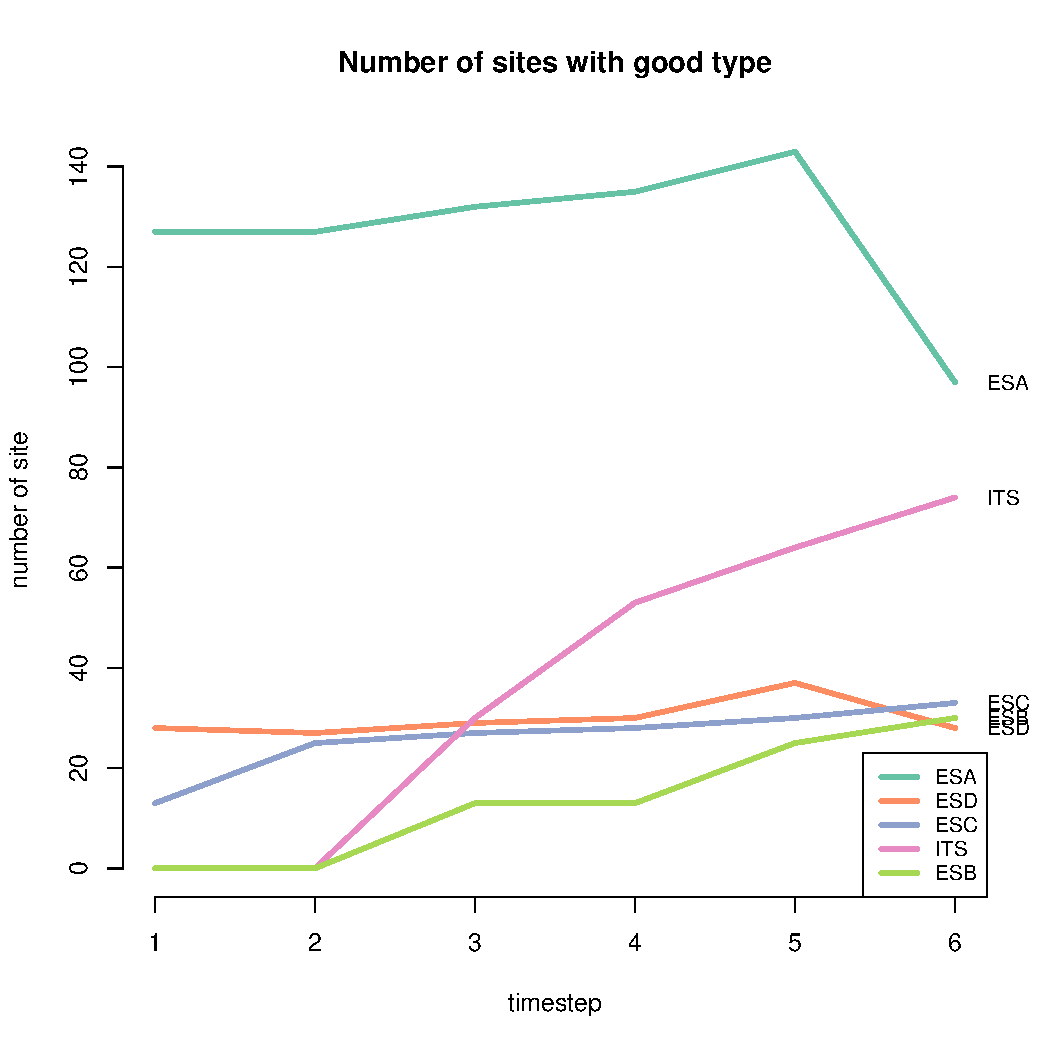
\includegraphics[width=.3\textwidth]{images/plotData.pdf}	&
	    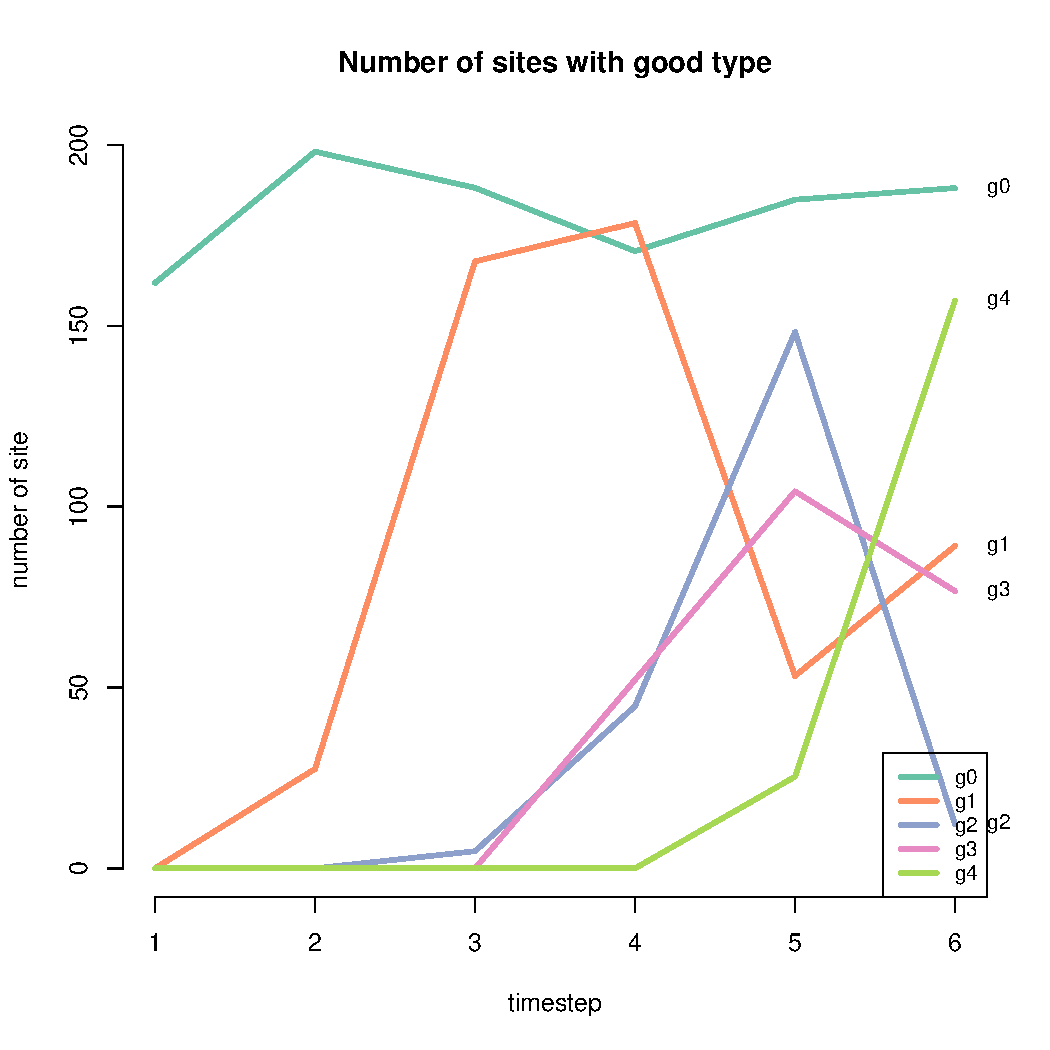
\includegraphics[width=.3\textwidth]{images/plotGoodSimu.pdf}	&
	    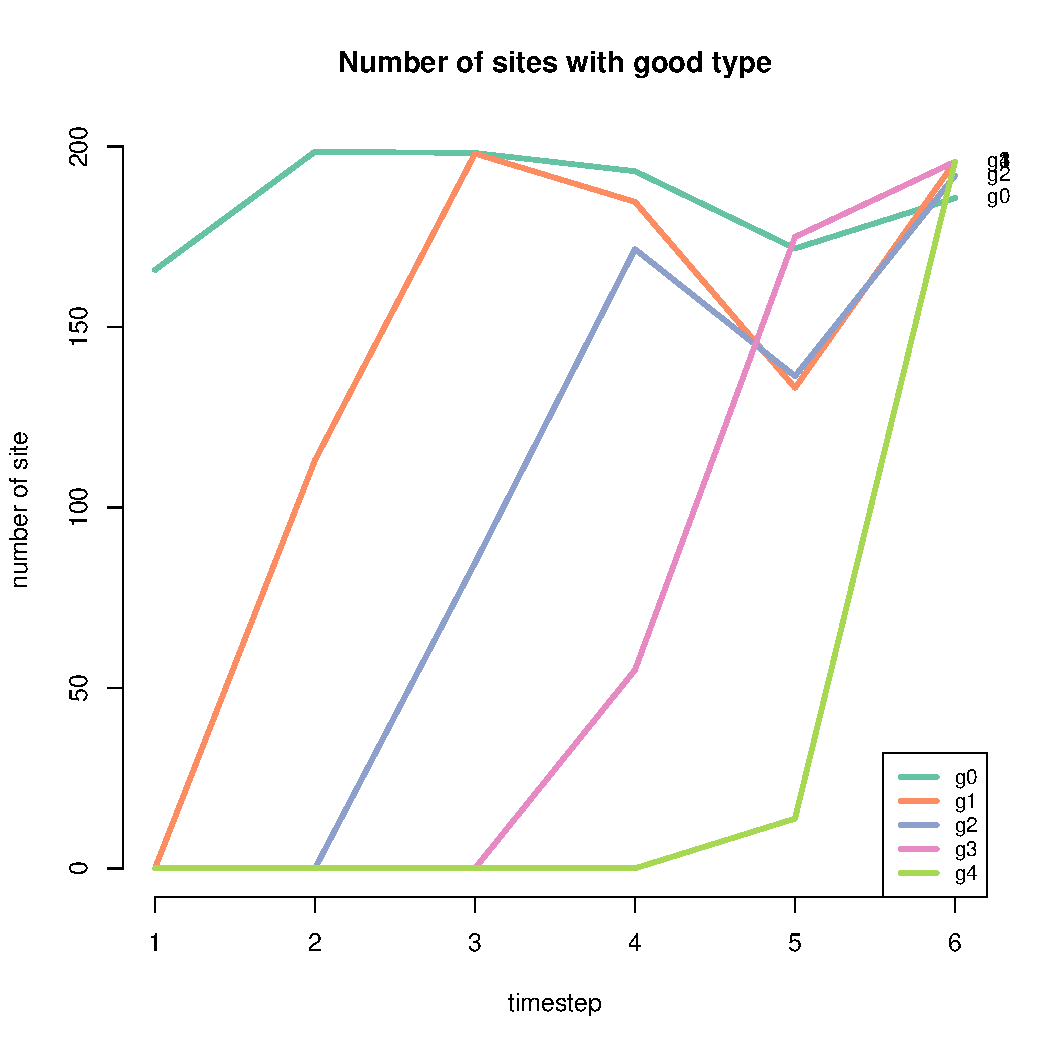
\includegraphics[width=.3\textwidth]{images/plotBadSimu.pdf}	\\

	\end{tabular}
    \end{table}
\end{frame}


\begin{frame}{Compare Simulations with Data}
    \centering
	    Data\\
	    \includegraphics<1>[width=.3\textwidth]{images/plotData.pdf}  
	    \includegraphics<2-4>[width=.3\textwidth]{images/plotData1.pdf}
	    \includegraphics<5-7>[width=.3\textwidth]{images/plotData2.pdf}
	    \includegraphics<8-10>[width=.3\textwidth]{images/plotData3.pdf}
	    \includegraphics<11-13>[width=.3\textwidth]{images/plotData4.pdf}
	    \includegraphics<14-16>[width=.3\textwidth]{images/plotData5.pdf}
	    \includegraphics<17->[width=.3\textwidth]{images/plotData.pdf}  

	\begin{tabular}{cc}
	    ExpG & ExpB\\
	    \includegraphics<1>[width=.3\textwidth]{images/plotGoodSimu.pdf}  

	    \includegraphics<2>[width=.3\textwidth]{images/plotGoodSimu1A.pdf}
	    \includegraphics<3>[width=.3\textwidth]{images/plotGoodSimu1B.pdf}
	    \includegraphics<4>[width=.3\textwidth]{images/plotGoodSimu1C.pdf}

	    \includegraphics<5>[width=.3\textwidth]{images/plotGoodSimu2A.pdf}
	    \includegraphics<6>[width=.3\textwidth]{images/plotGoodSimu2B.pdf}
	    \includegraphics<7>[width=.3\textwidth]{images/plotGoodSimu2C.pdf}

	    \includegraphics<8>[width=.3\textwidth]{images/plotGoodSimu3A.pdf}
	    \includegraphics<9>[width=.3\textwidth]{images/plotGoodSimu3B.pdf}
	    \includegraphics<10>[width=.3\textwidth]{images/plotGoodSimu3C.pdf}

	    \includegraphics<11>[width=.3\textwidth]{images/plotGoodSimu4A.pdf}
	    \includegraphics<12>[width=.3\textwidth]{images/plotGoodSimu4B.pdf}
	    \includegraphics<13>[width=.3\textwidth]{images/plotGoodSimu4C.pdf}

	    \includegraphics<14>[width=.3\textwidth]{images/plotGoodSimu5A.pdf}
	    \includegraphics<15>[width=.3\textwidth]{images/plotGoodSimu5B.pdf}
	    \includegraphics<16>[width=.3\textwidth]{images/plotGoodSimu5C.pdf}

	    \includegraphics<17>[width=.3\textwidth]{images/plotGoodSimu.pdf}  
	    \includegraphics<18>[width=.3\textwidth]{images/plotGoodSimuEnd.pdf}  

	    &

	    \includegraphics<1>[width=.3\textwidth]{images/plotBadSimu.pdf}  

	    \includegraphics<2>[width=.3\textwidth]{images/plotBadSimu1A.pdf}
	    \includegraphics<3>[width=.3\textwidth]{images/plotBadSimu1B.pdf}
	    \includegraphics<4>[width=.3\textwidth]{images/plotBadSimu1C.pdf}

	    \includegraphics<5>[width=.3\textwidth]{images/plotBadSimu2A.pdf}
	    \includegraphics<6>[width=.3\textwidth]{images/plotBadSimu2B.pdf}
	    \includegraphics<7>[width=.3\textwidth]{images/plotBadSimu2C.pdf}

	    \includegraphics<8>[width=.3\textwidth]{images/plotBadSimu3A.pdf}
	    \includegraphics<9>[width=.3\textwidth]{images/plotBadSimu3B.pdf}
	    \includegraphics<10>[width=.3\textwidth]{images/plotBadSimu3C.pdf}

	    \includegraphics<11>[width=.3\textwidth]{images/plotBadSimu4A.pdf}
	    \includegraphics<12>[width=.3\textwidth]{images/plotBadSimu4B.pdf}
	    \includegraphics<13>[width=.3\textwidth]{images/plotBadSimu4C.pdf}

	    \includegraphics<14>[width=.3\textwidth]{images/plotBadSimu5A.pdf}
	    \includegraphics<15>[width=.3\textwidth]{images/plotBadSimu5B.pdf}
	    \includegraphics<16>[width=.3\textwidth]{images/plotBadSimu5C.pdf}

	    \includegraphics<17>[width=.3\textwidth]{images/plotBadSimu.pdf}  
	    \includegraphics<18>[width=.3\textwidth]{images/plotBadSimuEnd.pdf}  
	    \\

	    \tiny
	    $\uncover<4->{\Delta_{ExpG} = A} \uncover<7->{ + B}\uncover<10->{ + C}\uncover<13->{ + D}\uncover<16->{ + E} \uncover<18->{ \approx 31} $ & 
	    \tiny 
	    $\uncover<4->{\Delta_{ExpB} = A'} \uncover<7->{ + B'}\uncover<10->{ + C'}\uncover<13->{ + D'}\uncover<16->{ + E'} \uncover<18->{ \approx 42} $ 





	\end{tabular}
	

    \end{frame}

\begin{frame}{Distribution of simulations scores}
    \begin{center}
	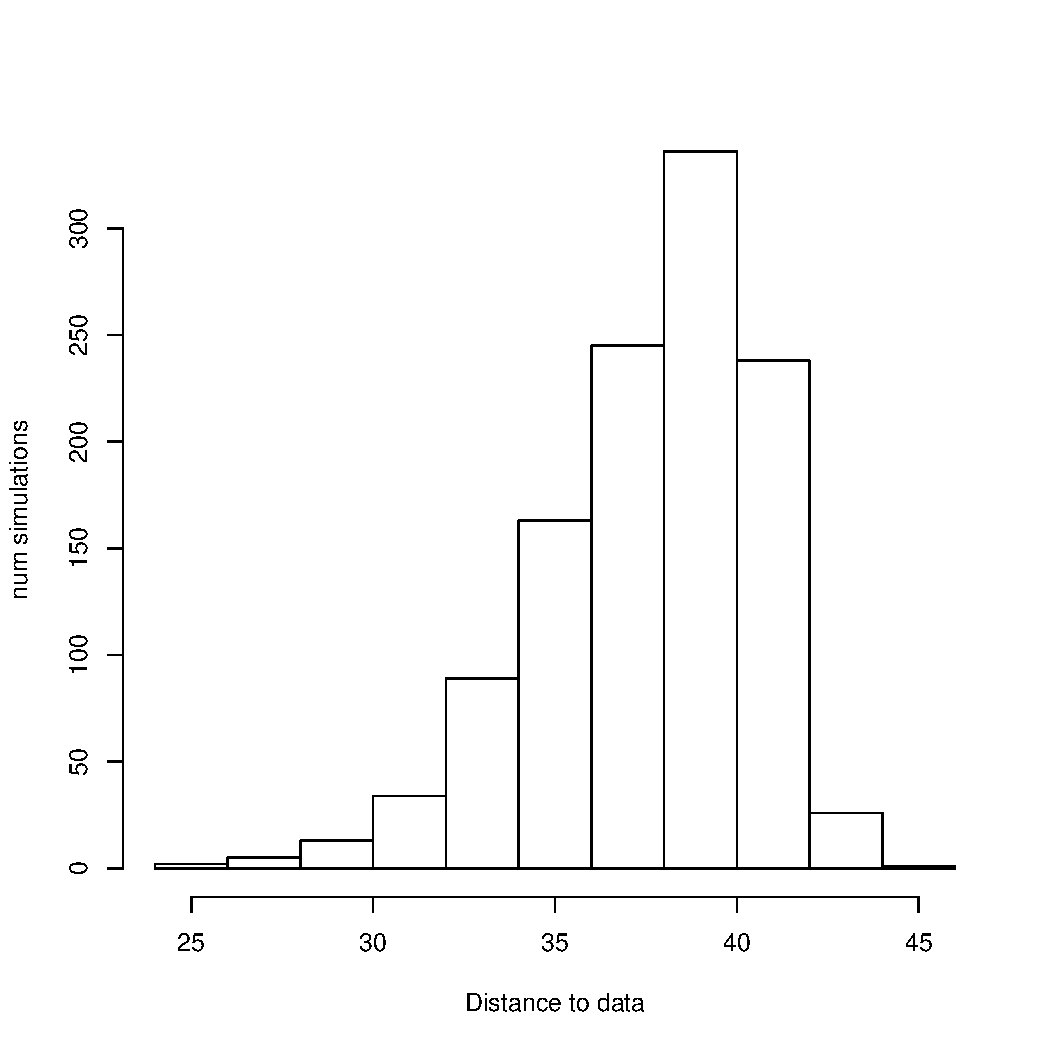
\includegraphics[width=.65\textwidth]{images/histScore.pdf}\\
    \end{center}
\end{frame}

\begin{frame}{Distribution of simulations scores}
    \begin{center}
	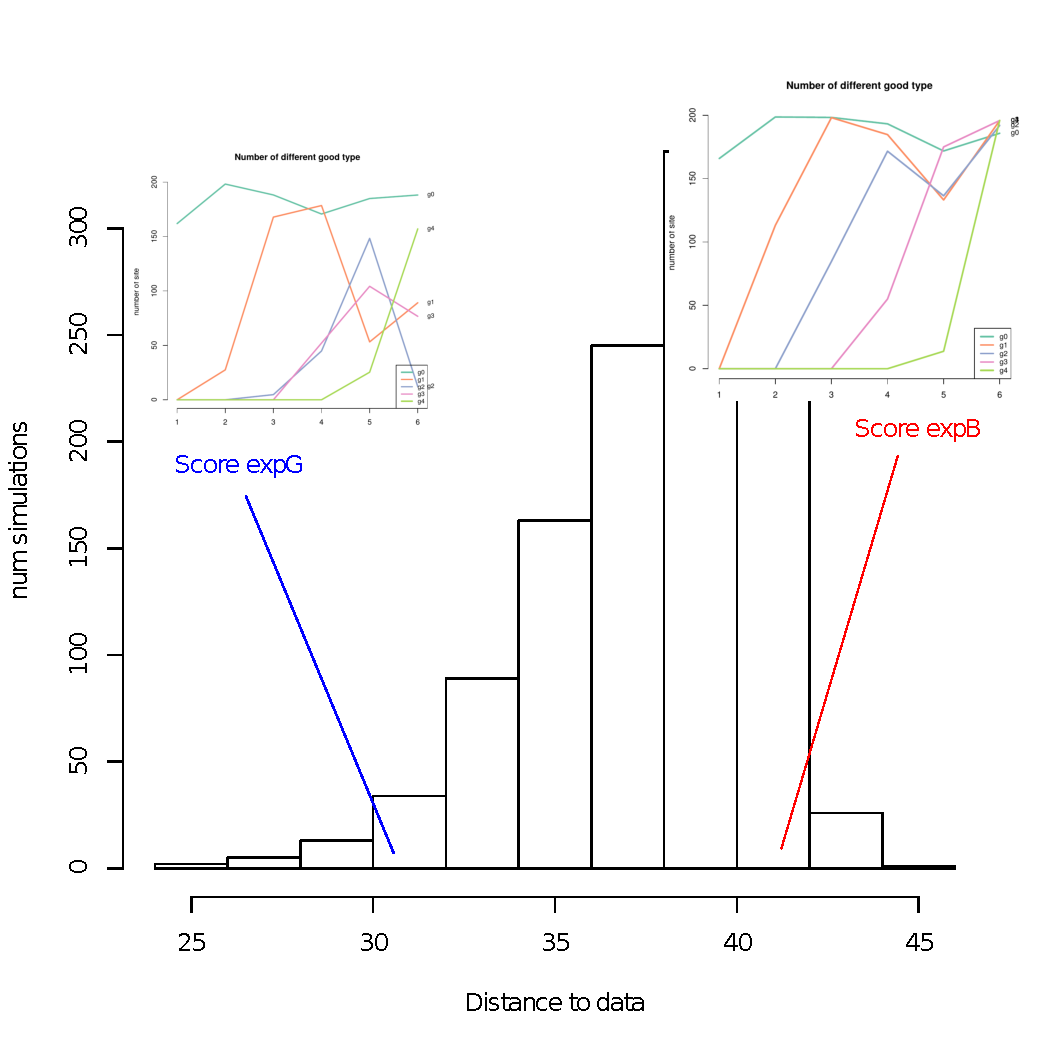
\includegraphics[width=.65\textwidth]{images/histScoreGB.pdf}\\
    \end{center}
\end{frame}

\begin{frame}{Compare pairs of parameters}

    \begin{center}
	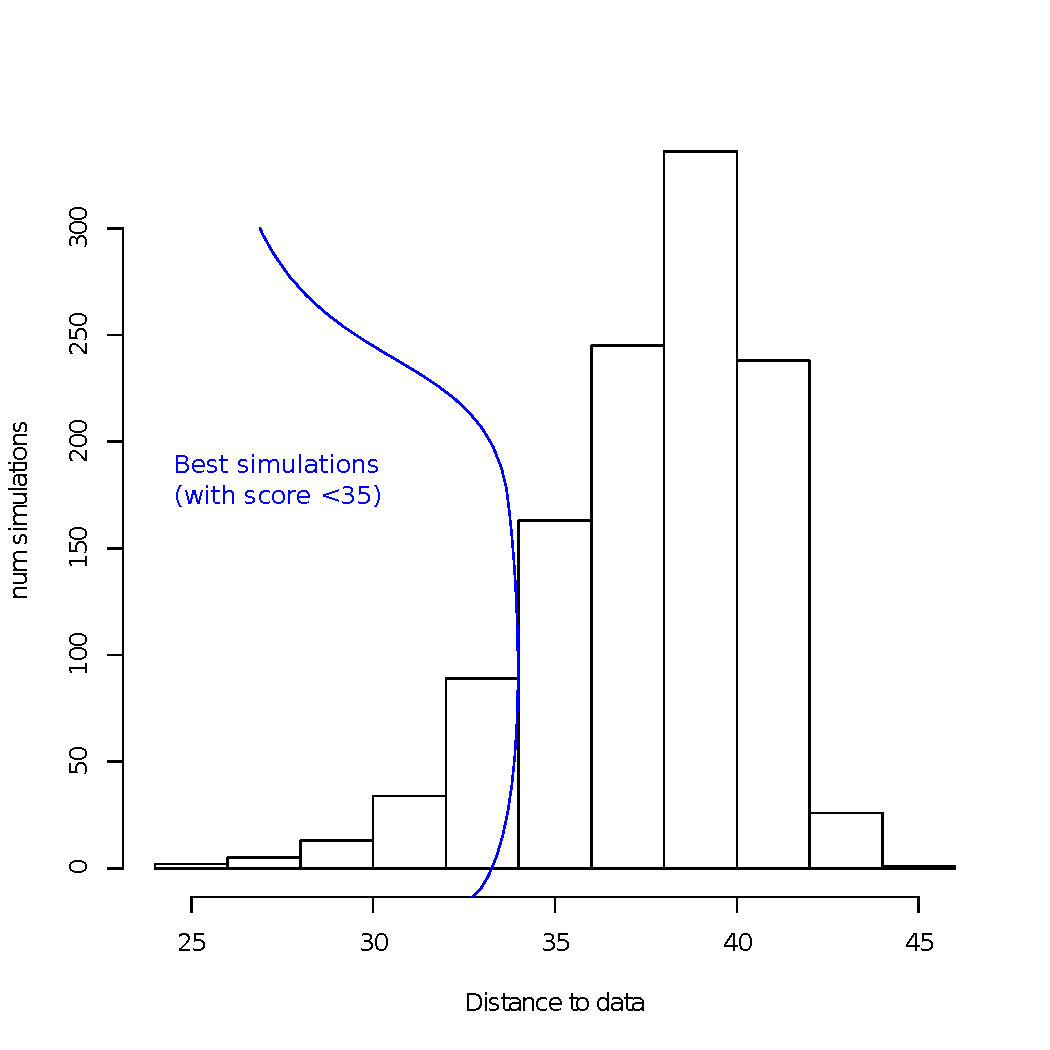
\includegraphics[width=.65\textwidth]{images/histScoreBest.pdf}\\
    \end{center}
    We select only the simulations ``more similar'' to the data.
\end{frame}

\begin{frame}{Compare pairs of parameters}
    For each pairs of parameters, we count how many simulations fall within this ``more similar'' threshold.
    \begin{figure}
	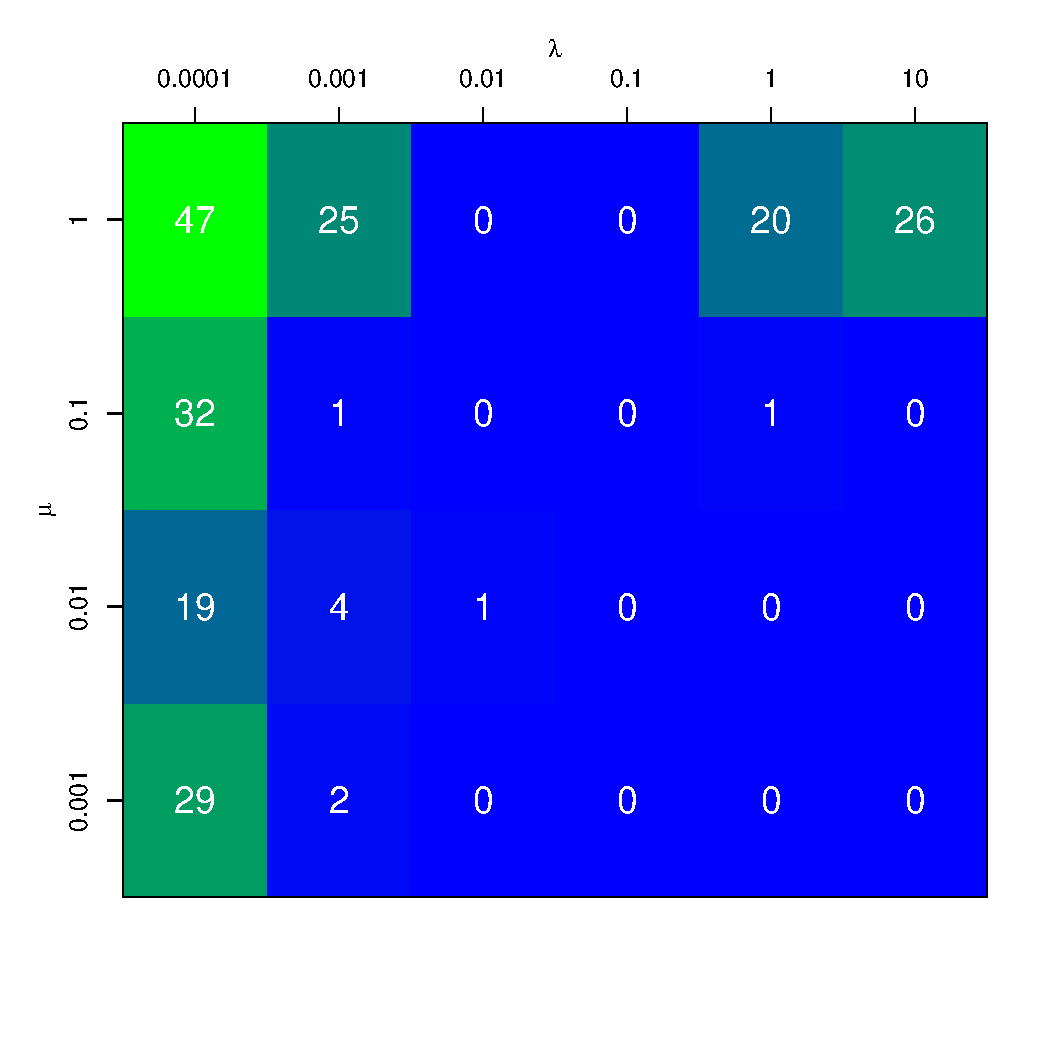
\includegraphics[width=.4\textwidth]{images/heatmapSimu}\\
	\centering
    \end{figure}

    \uncover<2->{Interpretation?
    \begin{itemize}
	\item <3-> Model not satisfying yet.
	\item <4-> \textcolor{UPF}{Very limited}
	\item <5-> But\dots
    \end{itemize}
}
\end{frame}

\begin{frame}{Interpretation}
    \begin{figure}
	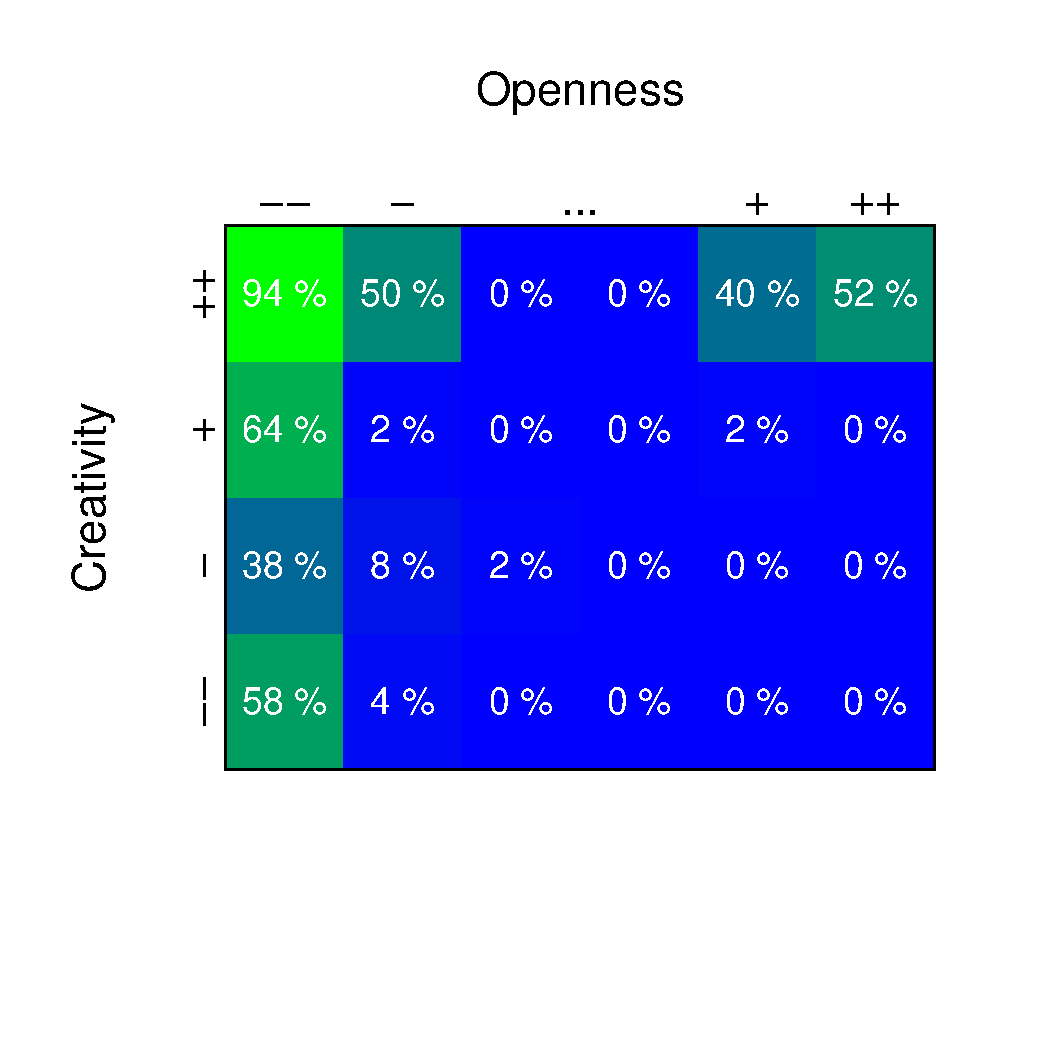
\includegraphics[width=.65\textwidth]{images/heatmapSimuProba.pdf}\\
	\centering
    \end{figure}

\end{frame}


%%%TODO
%\begin{frame}{Limitation}
%    (beside the fact that the model isn't satisfying us yet)\\
%    A way to compare hypothese:\\
%    \hspace{1cm}Previous example: 
%    \begin{itemize}
%	\item All assumptions can change those results
%	    \begin{itemize}
%		\item How we defined when ``a experiment \emph{reproduce} the data''
%		\item The data we are using
%
%	    \end{itemize}
%    \end{itemize}
%
%\end{frame}



\begin{frame}
	\begin{center}
		Thank you for you attention\\
%		What was the nature of Roman economy?\\
		\vspace{.5cm}
		\includegraphics[width=2cm]{images/LOGO-ERC.jpg} \hfil	\includegraphics[width=3cm]{../../logos/epnetLogo.png}\\
		
\includegraphics[width=3cm]{images/leverhulme}\\
		\vspace{.5cm}
		\scriptsize
			http://www.roman-ep.net/\\
			@simoncarrignon
	\end{center}


\end{frame}

\end{document}



